\documentclass{article}

%===============================
%
%          📦 Paquetes
%
%===============================

% === Configuración del documento y tipografía ===
\usepackage[a4paper, top=3cm, bottom=2.5cm, left=2.5cm, right=2.5cm]{geometry}
\usepackage[spanish]{babel}
\usepackage[utf8]{inputenc}
\usepackage[T1]{fontenc}
\usepackage{eulervm}



% === Gráficos y representaciones visuales ===
\usepackage{tikz}
\usepackage{pgfplots}
\pgfplotsset{compat=1.18}
\usepackage{graphicx}
\usepackage{subcaption}

% === Estilo y personalización ===
\usepackage{titling}
\usepackage{titlesec}
\usepackage{tocloft} 
\usepackage{fancyhdr}
\usepackage{setspace}
\usepackage{caption}

% === Matemáticas y símbolos ===
\usepackage{amsmath}
\usepackage{amssymb}
\usepackage{cancel}

% === Estructura y disposición del contenido ===
\usepackage{array}
\usepackage{multicol}
\usepackage{float}
\usepackage{indentfirst}

% === Hipervínculos y referencias ===
\usepackage{tocbibind}
\usepackage[colorlinks=true, linkcolor=black]{hyperref}

%===============================
%
%          ⬆️⬇️ Cabeceras
%
%===============================
\pagestyle{fancy}
\fancyhf{}
\fancyhead[L]{
\includegraphics[width=2.5cm,clip,trim=0cm 1cm 24cm 1cm]{assets/logo-utp.png}}
\vspace{0.5mm}\fancyhead[R]{\textit{Fundamentos de Electromagnetismo}\vspace{0.5mm}}
\fancyfoot[R]{\thepage}
\setlength{\headheight}{26.23502pt}
\addtolength{\topmargin}{-5.64944pt}

%======================================
%
%          📑 Espaciado de Párrafos
%
%======================================

\setlength{\parskip}{1.5em}
\setlength{\parindent}{0pt}

%======================================
%
%          📕 Estrucura del título
%
\title{
  \pagenumbering{gobble}
  \vspace{1cm}
  % 
\includegraphics[width=5cm,clip,trim=6cm 6cm 6cm 6cm]{./assets/isotipo.jpg} \\
  
\includegraphics[width=5cm,clip,trim=0cm 2.9cm 0cm 0cm]{./assets/isotipo-utp.png} \\
  \vspace{0.5cm}
  \textbf{Universidad Tecnológica del Perú} \\
  \vspace{0.5cm}
  \text{Investigación Académica} \\
  \vspace{1cm}
    {\huge \textbf{APF: Proyecto de Clasificación Automatizada Mediante Sensores Ópticos}} \\
  \vspace{1cm}
  % \large \textbf{Para acceder al título de...} \\
}
\author{
  \begin{tabular}{ll}
    \textbf{Acosta Luquillas Nathaly Esthefania} & \texttt{U23271317} \\
    \textbf{Fasabi Benavente Mirella del Rosario} & \texttt{U23254210} \\
    \textbf{Huatay Salcedo, Luis Elías} & \texttt{U24218809} \\
    \textbf{Reynoso Lazo Luis Alexander} & \texttt{U22233575} \\
    \textbf{Sigueñas Olivera Jordan Joel} & \texttt{U23314090} \\
    \textbf{Vicente Chaupis Jose Martin} & \texttt{U22207942} \\
    \textbf{Linares Fernández Bryan Josué} & \texttt{U22214029} \\
  \end{tabular} \\
  % \texttt{Ingeniería}\\
}

\bibliographystyle{plain} % estilos: plain, alpha, abbrv, unsrt, etc.


\begin{document}
% \date{14 de agosto de 2024}
\maketitle
\begin{center}
  Docente: \textbf{Pablo Andrés Villegas Chunga} \\
\end{center}

%======================================
%
%          📚 Inicio del documento
%
%======================================

\newpage

\begin{center}
\Large\bfseries Índice
\end{center}
\begingroup
\let\clearpage\relax
\renewcommand{\contentsname}{}
\tableofcontents
\endgroup


\newpage
% Inicio de la numeración de páginas (desde aquí)
\pagenumbering{arabic}
\setcounter{page}{1}  
\vspace*{\fill}

\section{Introducción}

  El presente proyecto tiene como finalidad aplicar la Metodología de Gestión de Proyectos Clásica, siguiendo el marco de trabajo propuesto por el Project Management Institute (PMI) y utilizando herramientas del Framework del PMBOK. Durante la primera parte de la unidad, se desarrollará un marco predictivo para la gestión de un proyecto empresarial, abarcando las fases de Iniciación y Planificación.

  Para ello, se seleccionará una empresa y área específica, describiendo su misión, visión y objetivos estratégicos, así como el alineamiento del proyecto con dichos objetivos. Posteriormente, se documentarán los procesos de iniciación (objetivos, alcance inicial, gestión de interesados y acta de constitución) y planificación (gestión de integración, alcance, cronograma, costes, calidad, recursos, comunicaciones, riesgos y adquisiciones).

  Finalmente, se presentará un informe detallado que incluya todos los elementos mencionados, demostrando la capacidad de aplicar la metodología de gestión de proyectos en un entorno empresarial real.

\vspace*{\fill}
\section{Descripción General}
Diseñar y construir un prototipo de sistema automatizado para la clasificación de mandarinas basado en su grado de madurez, utilizando sensores ópticos que operan bajo principios electromagnéticos para mejorar la eficiencia y objetividad del proceso de selección.

\section{Objetivos Específicos}
\begin{enumerate}
    \item Analizar las propiedades ópticas de las mandarinas para definir un criterio de madurez.
    \item Seleccionar y calibrar los componentes electrónicos (sensores, microcontrolador, actuadores).
    \item Diseñar e implementar una estructura mecánica para el transporte y clasificación.
    \item Desarrollar el software de control que toma las decisiones de clasificación.
    \item Validar el funcionamiento del prototipo integrado con pruebas reales.
\end{enumerate}

\section{Alcance del Proyecto}
Este proyecto busca demostrar, de manera práctica, cómo los principios del electromagnetismo y la visión por computadora pueden aplicarse en un sistema de clasificación de frutas. Para ello, se construyó una banda transportadora de 40 cm equipada con una cámara, una Raspberry Pi y servomotores que permiten identificar y separar mandarinas de acuerdo con su grado de madurez.

El alcance está enfocado en el desarrollo de un prototipo funcional a escala, utilizando materiales accesibles como MDF, motores DC y componentes electrónicos básicos. Con este sistema, se busca simular un proceso real de selección postcosecha, validando que con recursos limitados es posible diseñar soluciones automatizadas que mejoren la eficiencia y objetividad de la clasificación de productos agrícolas.

\section{Limitaciones}
\begin{itemize}
    \item El modelo está pensado para frutas simuladas o de prueba, no para cargas reales de gran tamaño o peso.
    \item El sistema funciona únicamente sobre superficies planas y estables, sin incorporar mecanismos de suspensión ni adaptación a diferentes terrenos.
    \item La automatización es básica: se centra en la detección de color para determinar madurez, sin integrar algoritmos avanzados de visión artificial ni sensores adicionales.
    \item La velocidad de operación es reducida, ya que se priorizó la estabilidad y el control del motor antes que la rapidez del transporte.
\end{itemize}

\section{Estructura del Proyecto}
El prototipo consiste en una banda transportadora de 40 cm de longitud diseñada para clasificar mandarinas simuladas según su grado de madurez.

El proceso de funcionamiento es el siguiente:
\begin{enumerate}
    \item Un motor DC transporta el fruto hasta la zona de análisis.
    \item Una cámara conectada a una Raspberry Pi 4 captura la imagen en tiempo real.
    \item Un programa en Python con la librería OpenCV analiza el color:
    \begin{itemize}
        \item Verde intenso o verde amarillento: fruto inmaduro.
        \item Amarillo o naranja brillante: fruto maduro.
    \end{itemize}
    \item Según la decisión, la Raspberry Pi activa uno de dos servomotores que desvían el fruto hacia el canal correspondiente.
\end{enumerate}

De esta manera, el sistema opera de forma autónoma, replicando un proceso real de selección postcosecha con tecnología accesible y de código abierto.

\begin{figure}[H]
    \centering
    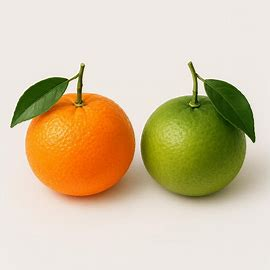
\includegraphics[width=0.7\textwidth]{./assets/mandarinas.jpeg}
    \caption{Mandarinas clasificadas según su grado de madurez en el prototipo.}
    \label{fig:mandarinas}
\end{figure}

\newpage
\section{Materiales y Componentes}

A continuación se detallan los materiales y componentes utilizados en la implementación del sistema de clasificación automática de frutas:

\begin{table}[H]
\centering
\caption{Lista de materiales y componentes del proyecto}
\begin{tabular}{|p{0.35\textwidth}|p{0.6\textwidth}|}
\hline
\textbf{Componente} & \textbf{Función en el sistema} \\
\hline
Raspberry Pi 4 (4 GB RAM) & Ejecuta código en Python, procesa imágenes de la cámara, toma decisiones de clasificación y controla sensores y motor. \\
\hline
Fuente de alimentación (5V/2A) & Alimenta la Raspberry Pi con la potencia necesaria para funcionar establemente. \\
\hline
Tarjeta microSD (16 GB+) & Almacena el sistema operativo (Raspberry Pi OS) y los programas en Python. \\
\hline
Webcam USB HD (o cámara Pi) & Captura imágenes en tiempo real de las frutas para que Python determine su grado de madurez. \\
\hline
Motor DC (con reductor 6V) & Impulsa el movimiento de la banda transportadora a velocidad controlada y constante. \\
\hline
Driver L298N & Actúa como interfaz entre la Raspberry Pi y el motor: permite controlar dirección y velocidad mediante señales PWM. \\
\hline
Banda transportadora (goma/elástico) & Superficie móvil que transporta las frutas desde la entrada hasta la zona de clasificación. \\
\hline
Rodillos (poleas) & Soportan y guían la banda; uno está conectado al motor para transmitir el movimiento. \\
\hline
Servomotor SG90 & Accionan brazos o compuertas que desvían frutas hacia el canal correcto según su clasificación (madura / no madura). \\
\hline
Canales de salida & Conductos inclinados que dirigen las frutas clasificadas a sus respectivos contenedores (ej. canal A = madura, canal B = no madura). \\
\hline
Fuente externa (6V-9V) & Alimenta motor y servos de forma independiente para evitar sobreexigir la Raspberry Pi y causar reset. \\
\hline
Protoboard & Permite conexiones temporales y organizadas entre Raspberry Pi, sensores, servos y driver sin soldadura. \\
\hline
Cables jumper & Conectan los pines GPIO de la Raspberry Pi con los componentes electrónicos vitales de control. \\
\hline
Base de MDF 40 cm & Soporte estructural que sostiene toda la maqueta: banda, motor, electrónica y canales. \\
\hline
Soporte para cámara & Mantiene la cámara fija y alineada sobre la zona de análisis para capturar imágenes claras y consistentes. \\
\hline
Frutas modelo (pintadas) & Simulan frutas reales con diferentes grados de madurez (verde = inmadura, amarillo/naranja = madura) para probar el sistema. \\
\hline
\end{tabular}
\end{table}

\subsection{Materiales de Soporte y Estructura}

\begin{itemize}
    \item \textbf{MDF de 3mm}: Para la estructura base y soportes del sistema
    \item \textbf{Silicona caliente}: Para fijación de componentes electrónicos y refuerzo estructural
    \item \textbf{Tornillos y tuercas}: Para ensamblaje mecánico de la estructura
    \item \textbf{Pegamento para madera}: Para uniones estructurales permanentes
\end{itemize}

\subsection{Herramientas Utilizadas}

\begin{itemize}
    \item Cortadora láser para corte preciso del MDF
    \item Destornilladores para ajuste de componentes mecánicos
    \item Taladro manual para perforaciones adicionales
    \item Soldador para conexiones eléctricas del portapilas
    \item Instrumentos de medición y trazado (reglas, lápiz, tijera)
\end{itemize}

\begin{multicols}{2}
  \section*{Fundamentos Básicos de Electricidad}

\begin{enumerate}
    \item \textbf{Carga eléctrica}  
    La carga eléctrica es una propiedad fundamental de la materia.  
    \[
        q = n \cdot e
    \]  
    donde \( q \) es la carga eléctrica, \( n \) el número de electrones (o protones) y \( e = 1.6 \times 10^{-19}\,\text{C} \).

    \item \textbf{Ley de Coulomb}  
    La fuerza entre dos cargas puntuales es:  
    \[
        F = k_e \frac{|q_1 q_2|}{r^2}
    \]  
    donde \( k_e = 8.99 \times 10^9 \,\text{N·m}^2/\text{C}^2 \), \( q_1 \) y \( q_2 \) son las cargas, y \( r \) la distancia entre ellas.

    \item \textbf{Campo eléctrico}  
    Definición de campo debido a una carga puntual:  
    \[
        \vec{E} = \frac{\vec{F}}{q} = k_e \frac{q}{r^2} \,\hat{r}
    \]  

    \item \textbf{Superposición de campos eléctricos}  
    El campo total en un punto es la suma vectorial de los campos individuales:  
    \[
        \vec{E}_{\text{total}} = \sum_i \vec{E}_i
    \]

    \item \textbf{Energía potencial eléctrica}  
    La energía potencial entre dos cargas:  
    \[
        U = k_e \frac{q_1 q_2}{r}
    \]  

    \item \textbf{Potencial eléctrico}  
    El potencial en un punto debido a una carga puntual:  
    \[
        V = k_e \frac{q}{r}
    \]  
    y su relación con el campo eléctrico es:  
    \[
        \vec{E} = - \nabla V
    \]

    \item \textbf{Diferencia de potencial (voltaje)}  
    La diferencia de potencial entre dos puntos \(A\) y \(B\):  
    \[
        \Delta V = V_B - V_A = - \int_A^B \vec{E} \cdot d\vec{l}
    \]

    \item \textbf{Capacitancia}  
    Definida como la relación entre la carga y el voltaje:  
    \[
        C = \frac{Q}{V}
    \]  
    Para un capacitor de placas paralelas:  
    \[
        C = \varepsilon \frac{A}{d}
    \]  
    donde \( \varepsilon \) es la permitividad del material, \( A \) el área de las placas y \( d \) la distancia entre ellas.

    \item \textbf{Energía almacenada en un capacitor}  
    La energía se expresa como:  
    \[
        U = \frac{1}{2} C V^2
    \]
\end{enumerate}
\end{multicols}
\newpage

\section{Prototipo}

Nuestro prototipo de clasificación automática de frutas se basa en una banda transportadora accionada por un motor DC, controlada por una Raspberry Pi 4 que procesa imágenes capturadas por una cámara para determinar el grado de madurez de las frutas. Según el análisis de color, la Raspberry Pi activa servomotores que desvían las frutas hacia canales específicos.

\begin{figure}[H]
    \centering
    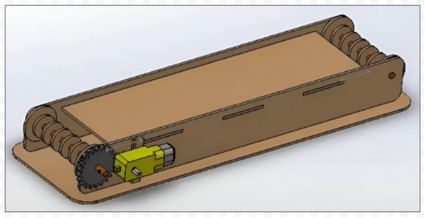
\includegraphics[width=0.8\textwidth]{./assets/prototipo.png}
    \caption{Prototipo de clasificación automática de frutas.}
    \label{fig:prototipo}
\end{figure}

\textbf{Maqueta:} La estructura está construida con MDF de 3mm, con una base de 40 cm que soporta la banda transportadora, el motor, la cámara y los canales de salida. La banda es de goma para un buen agarre de las frutas.

\begin{figure}[H]
    \centering
    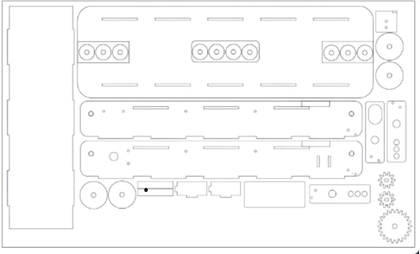
\includegraphics[width=0.7\textwidth]{./assets/maqueta.png}
    \caption{Maqueta del sistema de clasificación automática de frutas.}
    \label{fig:maqueta}
\end{figure}

A continuación puede revisar el video demostrativo del funcionamiento del prototipo:

\begin{center}
    \textbf{Video demostrativo:}  
    \href{https://utpedupe-my.sharepoint.com/:v:/g/personal/u22233575_utp_edu_pe/ESdkn_1TnllGkt0cGerWwMgBXVQGKYCcalTcEf6V_v72PA?nav=eyJyZWZlcnJhbEluZm8iOnsicmVmZXJyYWxBcHAiOiJPbmVEcml2ZUZvckJ1c2luZXNzIiwicmVmZXJyYWxBcHBQbGF0Zm9ybSI6IldlYiIsInJlZmVycmFsTW9kZSI6InZpZXciLCJyZWZlcnJhbFZpZXciOiJNeUZpbGVzTGlua0NvcHkifX0&e=CYh8pB }{Ver video}
\end{center}

\subsection{Materiales:}

\begin{itemize}
    \item \textbf{Madera MDF 3mm}: Material principal para la estructura y base del prototipo.
    \item \textbf{Porta pilas}: Soporte para las pilas que alimentan el motor y otros componentes.
    \item \textbf{Motor reductor 3V (200RPM)}: Motor DC con reducción para accionar la banda transportadora.
    \item \textbf{Pilas AA}: Fuente de energía para el motor y servomotores.
    \item \textbf{Palillos de 5mm}: Utilizados como ejes o soportes en la estructura mecánica.
    \item \textbf{Corrospum negro}: Material para canales, separadores o soporte adicional.
    \item \textbf{Cables de calibre 24 AWG}: Para conexiones eléctricas entre componentes.
    \item \textbf{Switch}: Interruptor para encender o apagar el sistema de forma segura.
\end{itemize}





\bibliography{biblio} % sin extensión .bib

\end{document}